
%%%%%%%%%%%%%%%%%%%%%%% file typeinst.tex %%%%%%%%%%%%%%%%%%%%%%%%%
%
% Author: Mauricio Matamoros
% Updated: Oct 31, 2022
% Contact: mauricio@robocupathome.org
%
% This is the LaTeX source for the TDPTemplate using
% the LaTeX document class 'llncs.cls' Springer LNAI format
% used in the RoboCup Symposium submissions.
% http://www.springer.com/computer/lncs?SGWID=0-164-6-793341-0
%
% It may be used as a template for your own TDP - copy it
% to a new file with a new name and use it as the basis
% for your Team Description Paper
%
% NB: the document class 'llncs' has its own and detailed documentation, see
% ftp://ftp.springer.de/data/pubftp/pub/tex/latex/llncs/latex2e/llncsdoc.pdf
%
% Remark: Last page with specs won't be included in Camera ready TDP's.
%
% CHKTEX-FILE 8
% CHKTEX-FILE 13
%
%%%%%%%%%%%%%%%%%%%%%%%%%%%%%%%%%%%%%%%%%%%%%%%%%%%%%%%%%%%%%%%%%%%

\documentclass[runningheads,a4paper]{llncs}

% XeLaTeX support
\usepackage{ifxetex}
\ifxetex%
	\usepackage{fontspec}
	\usepackage{polyglossia}
	\setmainlanguage{english}
\else
	\usepackage[utf8]{inputenc}
	\usepackage[T1]{fontenc}
	\usepackage[english]{babel}
\fi

% Common packages
\usepackage{amsmath}
\usepackage{amssymb}
\setcounter{tocdepth}{3}
\usepackage{url}
\usepackage{float}
% \usepackage{titling}
\usepackage{wrapfig}
\usepackage{booktabs}
\usepackage{csquotes}
\usepackage{fancyhdr}
\usepackage{graphicx}
\usepackage{subcaption}
\usepackage{lastpage}
\usepackage[all]{nowidow}
\usepackage[inline]{enumitem}
\usepackage[usenames,dvipsnames]{xcolor}

% Referencing packages
\usepackage{varioref}
\usepackage[hidelinks]{hyperref}
\usepackage[noabbrev,nameinlink]{cleveref}

% \usepackage{lipsum}
\newcommand{\mytitle}{Chief Scientist Office 2024 Team Description Paper}
\newcommand{\myauthor}{Takaaki Numai, Airi Yokochi, Joshua Supratman, Tatsuro Sakaguchi, Yushi, Kaida, Gakuto Okamoto}

\newcommand{\robospecs}{%
	\newpage%
	\pagenumbering{gobble}%
	\pagestyle{fancy}%
	\fancyhf{}%
	\lhead{}%
	\chead{\footnotesize\myauthor\ | \footnotesize\mytitle}%
	\rhead{}%
	\rfoot{Robot software and hardware specification sheet}%
}

\newcommand{\BnL}[1][1em]{ \includegraphics[width=#1]{images/bnl.jpg} }




%%%%%%%%%%%%%%%%%%%%%%%%%%%%%%%%%%%%%%%%%%%%%%%%%%%%%%%%%%%%%%%%%%%%%%%%%%%%%%%%%%%%
%
% Title
%
%%%%%%%%%%%%%%%%%%%%%%%%%%%%%%%%%%%%%%%%%%%%%%%%%%%%%%%%%%%%%%%%%%%%%%%%%%%%%%%%%%%%

\title{Chief Scientist Office 2024 Team Description Paper}

\author{Takaaki Numai \and Airi Yokochi \and Joshua Supratman \and Tatsuro Sakaguchi \and Yushi Kaida \and Gakuto Okamoto\thanks{The order of authors is based on age.}}
\institute{SoftBank Corp. Chief Scientist Office \\
	\texttt{https://www.robocup.ros-sier.com/, https://github.com/sbgisen}}


\begin{document}
\maketitle
%%%%%%%%%%%%%%%%%%%%%%%%%%%%%%%%%%%%%%%%%%%%%%%%%%%%%%%%%%%%%%%%%%%%%%%%%%%%%%%%%%%%
%
% Abstract
%
%%%%%%%%%%%%%%%%%%%%%%%%%%%%%%%%%%%%%%%%%%%%%%%%%%%%%%%%%%%%%%%%%%%%%%%%%%%%%%%%%%%%

\begin{abstract}
	This paper presents SoftBank Corp. Japan team Chief Scientist Office’s new mobile manipulator “SOAR” for RoboCup 2024 @Home Open Platform League.
	Differing from our previous participation with “Cuboid-X,” a robot assembled from commercial products, SOAR integrates both custom-developed and commercial components, a significant step toward developing a customizable and affordable robotic platform.
	Our main achievement this year has been the successful integration of various hardware components and software development to tackle RoboCup challenges.

	Our approach includes detailed hardware design and calibration, such as the arm and the sensor-rich head.
	The software focuses on developing systems, such as object and speech recognition, tailored to the dynamic environment of RoboCup.

	SOAR embodies our vision of a robotic system that combines modularity with cost-effectiveness.
	As we continue to refine SOAR’s capabilities further, we are optimistic about its potential to create an adaptable, cost-effective robotic platform for a variety of applications and fields.

\end{abstract}


%%%%%%%%%%%%%%%%%%%%%%%%%%%%%%%%%%%%%%%%%%%%%%%%%%%%%%%%%%%%%%%%%%%%%%%%%%%%%%%%%%%%

\section{Introduction}
This paper details the RoboCup @Home Open Platform League team Chief Scientist Office from SoftBank Corp. Japan.
This is our second appearance at RoboCup @Home Open Platform League.
Since our last participation in 2022, we have made significant improvements, which include the introduction of our new mobile manipulator “SOAR.”

At SoftBank Corp. Chief Scientist Office, we aim to pioneer a customizable and affordable commercial robot platform akin to the modular ease found in computer assembly or the historical T-Ford model.
Our mission is to democratize robotics, making it accessible and adaptable for research and commercial use.
We believe in a future where integrating robotics into business is as straightforward as selecting components for a custom PC build.
With SOAR as a stepping stone, we aim to develop a versatile platform that celebrates modularity in both hardware and software, allowing seamless integration and upgrades through a suite of interchangeable modules.

\subsection{Focus of research}
Our research is motivated by the ambition to develop a customizable and affordable robot platform.
We recognize the constraints of current technologies and are committed to exploring their limits and potential. Key areas of our interest include but are not limited to:
\begin{itemize}
	\item Modularity and Configurability: Investigate how to design a system that allows for easy integration and customization of hardware modules.
	\item Device Integration: Tackling the hardware challenges related to the seamless integration of diverse devices and components
\end{itemize}
We believe that these research areas are crucial to bridging the gap between the aspirational and the practical, laying the groundwork for a robot that can adapt to various needs.

\section{Hardware Modules}
SOAR is a mobile manipulator comprising four main components: the mobile base, the torso, the manipulator, and the head as shown in Fig. \ref{fig:components}.
The mobile base and the manipulator are commercially available products, while the torso and the head are custom-developed by our team.
The head and the torso are separate components designed for specific functionalities; we designed the head to accommodate various interchangeable sensors and the torso to enhance the manipulator's reach and versatility.
All components are designed with minimal cable protrusion, with circuits centralized on the torso, thus streamlining the connection across components with minimal cabling.
This modular approach not only facilitates customization but also organizes and simplifies maintenance and upgrades, allowing for the interchange of components as needed.

\begin{figure}[tbp]
	\centering
	\begin{subfigure}[b]{0.4\linewidth}
		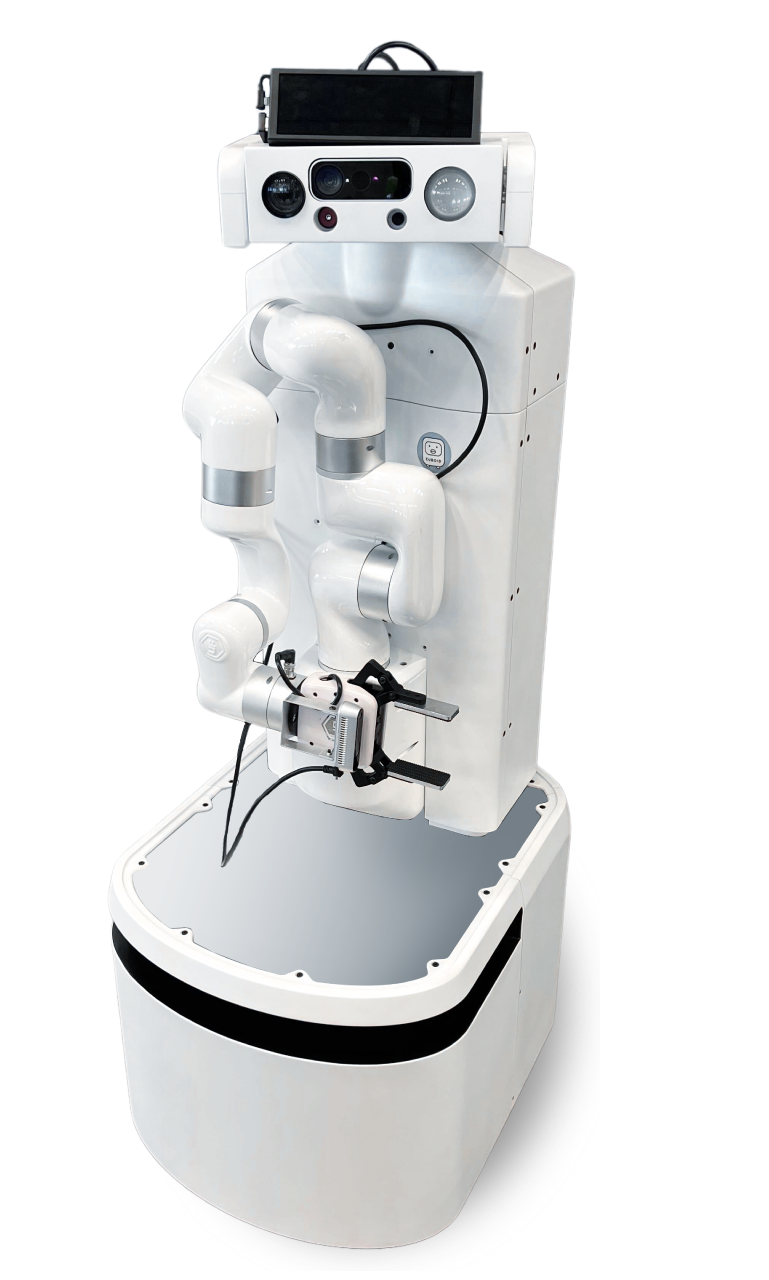
\includegraphics[width=\linewidth]{images/soar.png}
		\caption{SOAR.}
		\label{fig:component_soar}
	\end{subfigure}
	\begin{minipage}[b]{0.25\linewidth}
		\centering
		\begin{subfigure}[b]{\linewidth}
			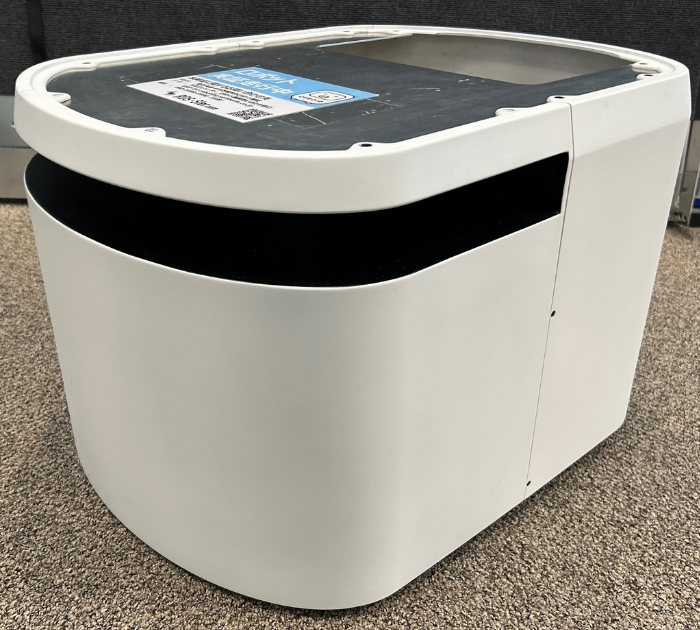
\includegraphics[width=\linewidth]{images/component_base.png}
			\caption{Mobile Base.}
			\label{fig:component_base}
		\end{subfigure}
		\begin{subfigure}[b]{\linewidth}
			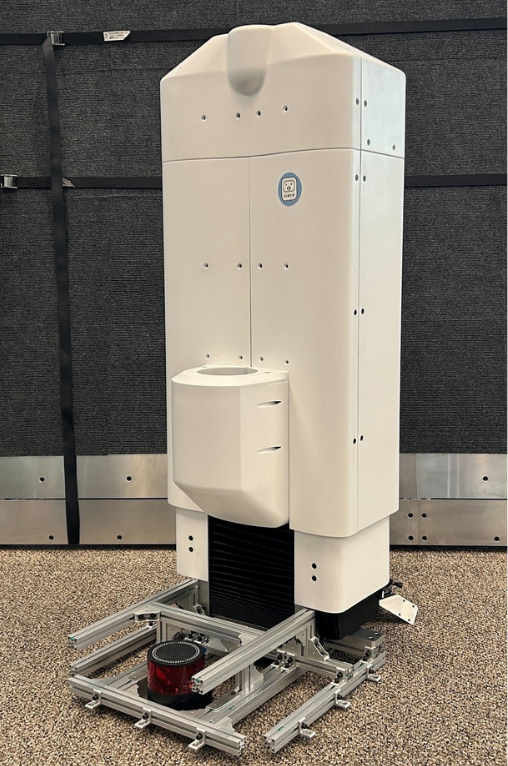
\includegraphics[width=\linewidth]{images/component_torso.png}
			\caption{Torso.}
			\label{fig:component_torso}
		\end{subfigure}
	\end{minipage}
	\hspace{0.01\linewidth}
	\begin{minipage}[b]{0.25\linewidth}
		\centering
		\begin{subfigure}[b]{\linewidth}
			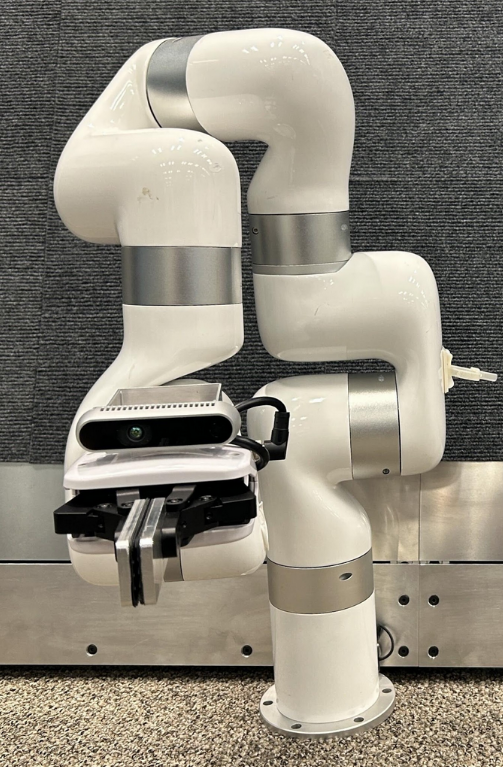
\includegraphics[width=\linewidth]{images/component_manipulator.png}
			\caption{Manipulator.}
			\label{fig:component_arm}
		\end{subfigure}
		\begin{subfigure}[b]{\linewidth}
			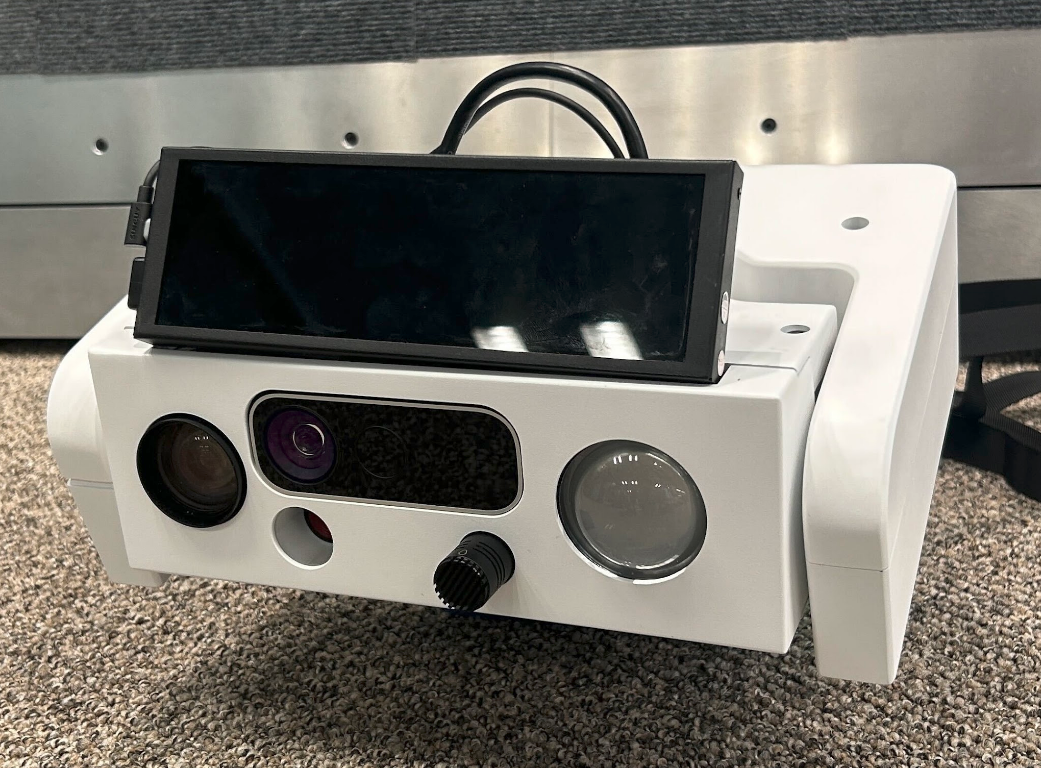
\includegraphics[width=\linewidth]{images/component_head.png}
			\caption{Head.}
			\label{fig:component_head}
		\end{subfigure}
	\end{minipage}
	\caption{SOAR and its four components.}
	\label{fig:components}
\end{figure}

\subsection{Mobile Base}
SOAR’s mobile base (Fig. \ref{fig:component_base}) is a 2-wheel differential drive mobile base developed by F-Design\footnote{\url{https://f-ds.jp/}}.
It is supplemented with two casters, and each driving wheel and caster are equipped with suspensions for smoother movement and stability.
We made additional modifications to the component, equipping it with a battery management system and a docking charging connector, enabling SOAR to recharge its battery autonomously once depleted, enhancing its operational autonomy and efficiency.
We connect the motor drivers and the battery management system to a USB hub, resulting in only two cables extending out: the USB cable from the device hub and the power supply cable.

\subsection{Torso}
The torso (Fig. \ref{fig:component_torso}), developed by our team, is a linear actuator with one degree of freedom equipped with a constant-force spring to provide gravity compensation.
The component elevates the head and the manipulator, providing a clearance of 410 mm, significantly enhancing the latter's reach and versatility.
In addition, the component also stores the main PC and controller box as it serves as the central hub for SOAR's hardware components.

\subsection{Manipulator}
The manipulator (Fig. \ref{fig:component_arm}) is xArm 7\footnote{\url{https://www.ufactory.cc/xarm-collaborative-robot/}}, a commercially available product developed by uFactory.
The end-effector is equipped with a two-finger gripper and a RGB-D hand camera.

\subsection{Head}
The head (Fig. \ref{fig:component_head}), designed as a sensory and interactive hub, supports a range of sensors and user interface devices for environmental understanding and social interaction.
Equipped with a USB hub for efficient cable management and a separate USB for the high-bandwith depth camera, it allows for easy swapping of sensors and devices, ensuring that the component can be customized for specific requirements.
The head extends three specific cables: a USB cable from the sensor hub, a separate USB for the depth camera, and a power supply cable.
In addition, the head has 2 degrees of freedom for pan and tilt movements, enhancing its SOAR’s ability to survey diverse environments and engage in social interaction more effectively.
Homing sensors have been integrated on both the pan and tilt for calibration and homing to enhance the head's functionality, eliminating the need for absolute encoders in motors, which reduces spatial requirements, eliminates the need for mechanical adjustments to achieve a homing position, and increases the flexibility in motor selection.

\section{Alignment Between Modules}
SOAR's modular design brings forth unique challenges in ensuring precise alignment between its components, mainly due to the frequent installation and removal of components during maintenance and upgrades, leading to performance variability.
The interchangeability of modules requires a robust system to maintain consistent performances across different configurations.

To address these challenges, we used the \text{robot\_calibration}\cite{ferguson2015robust} ROS package.
This package automatically fine-tuned the alignments of SOAR's components, ensuring each module aligns correctly with the system to maintain the robot's performance, significantly reducing the need to adjust the components to align with the system manually.
Figure \ref{fig:calibration}, shows an example with the manipulator and the head, where the measured joints align with their actual physical counterpart.
While we achieve good calibration results with the manipulator, calibrating other components, like the mobile base, presents more challenges and is an ongoing process to achieve the desired level of alignment and performance.

\begin{figure}[tbp]
	\centering
	\begin{subfigure}[t]{0.49\linewidth}
		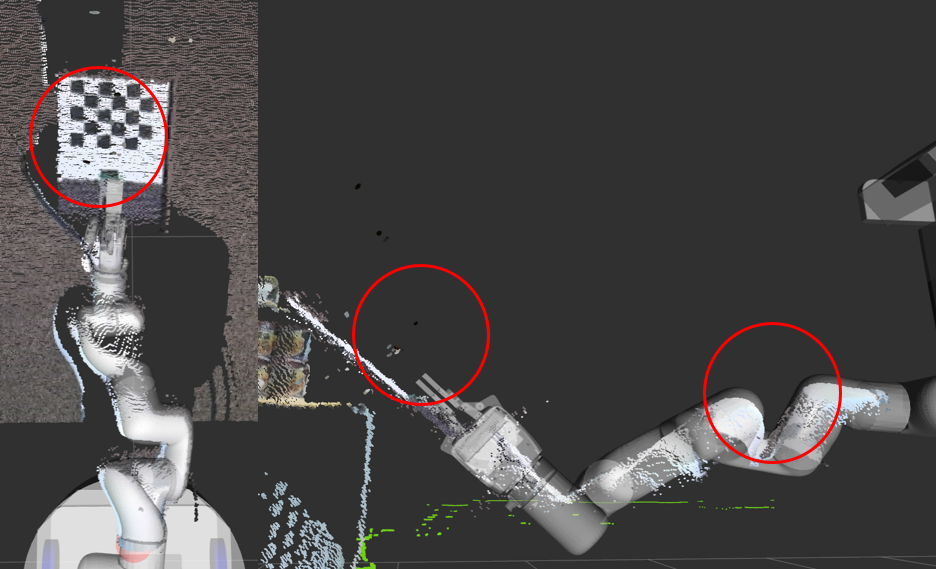
\includegraphics[width=\linewidth]{images/calibration_before.png}
		\caption{Before calibration. Red circles show the discrepancies between the measured joint and the actual joint.}
	\end{subfigure}
	\hfill
	\begin{subfigure}[t]{0.49\linewidth}
		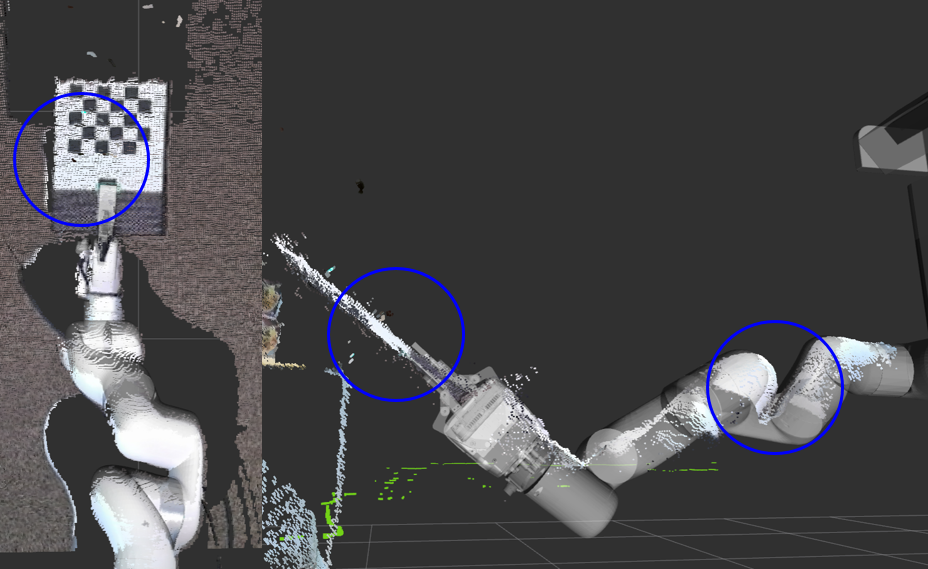
\includegraphics[width=\linewidth]{images/calibration_after.png}
		\caption{After calibration. Blue circles show the alignment between the measured joint and the actual joint, indicating improved accuracy and precision in the measurement.}
	\end{subfigure}
	\caption{Calibration results.}
	\label{fig:calibration}
\end{figure}

\section{Software}
The overview of our software system, shown in Fig. \ref{fig:overview} is comprised of three main layers:
\begin{enumerate}
	\item The perception layer, a collection of software modules that take the robot’s sensor data and process them to create a symbolic representation of the environment,
	\item the planning layer, a collection of software modules that take the state of the environment to evaluate and generate a sequence of appropriate robot behaviors, and
	\item the control layer, the collection of software modules that translates the planned behavior and sends appropriate commands to the actuators for the robot to interact with the environment
\end{enumerate}
The primary framework for software module interaction is Robot Operating System (ROS)\footnote{\url{https://www.ros.org/}}, with each software module representing one or several ROS nodes.

\begin{figure}[tbp]
	\centering
	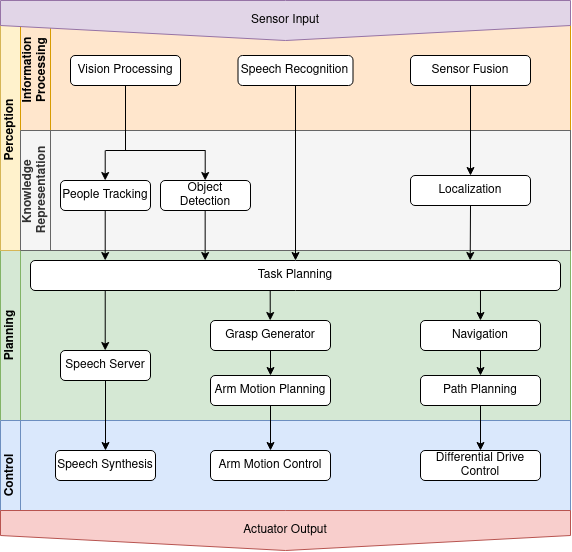
\includegraphics[width=0.7\linewidth]{images/software_overview.png}
	\caption{SOAR software overview.}
	\label{fig:overview}
\end{figure}

\subsection{Object Recognition}
Object detection and 3D localization are handled through the seamless integration of existing technologies.
We employed ultranlytics’s YOLOv8\cite{yolov8_ultralytics} for its object recognition capabilities, producing bounding boxes with labels for each detected object in the robot’s field of view.
To understand the object’s spatial orientation and structure, we used the \text{jsk\_pcl\_ros}\footnote{\url{https://github.com/jsk-ros-pkg/jsk\_recognition}} package for its robust point cloud processing.
We used the EuclideanClustering and the ClusterPointIndicesDecomposer functionalities within this package to segment and cluster point cloud data within the detected bounding boxes from YOLOv8 and generate 3D collision boxes along with its pose.
The pipeline is illustrated in Fig. \ref{fig:object_detection_pipeline}.

\begin{figure}[tbp]
	\centering
	\begin{subfigure}[t]{0.32\linewidth}
		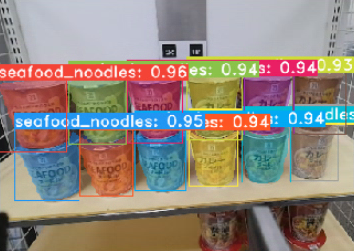
\includegraphics[width=1.0\linewidth]{images/object_detection_pipeline1.png}
		\caption{Detecting cup noodles with YOLOv8.}
		\label{fig:object_detection_pipeline1}
	\end{subfigure}
	\begin{subfigure}[t]{0.32\linewidth}
		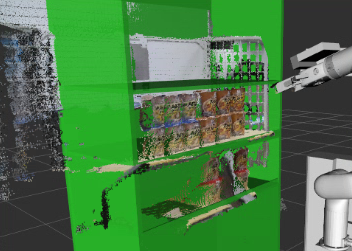
\includegraphics[width=1.0\linewidth]{images/object_detection_pipeline2.png}
		\caption{Point cloud data and MoveIt planning scene.}
		\label{fig:object_detection_pipeline2}
	\end{subfigure}
	\begin{subfigure}[t]{0.32\linewidth}
		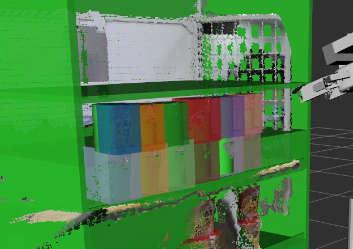
\includegraphics[width=1.0\linewidth]{images/object_detection_pipeline3.png}
		\caption{3D collision boxes generated by \text{jsk\_pcl\_ros} package.}
		\label{fig:object_detection_pipeline3}
	\end{subfigure}
	\caption{Object detection pipeline. YOLOv8's bounding box (Fig. \ref{fig:object_detection_pipeline1}) and the point cloud data (Fig. \ref{fig:object_detection_pipeline2}) are given to \text{jsk\_pcl\_ros} package to generate 3D collision boxes (Fig. \ref{fig:object_detection_pipeline3}), which are passed to MoveIt planning scene.}
	\label{fig:object_detection_pipeline}
\end{figure}

\subsection{Creating dataset}
To train YOLOv8 for object recognition in the dynamic nature of RoboCup competitions, where new objects are often introduced on the day of the event, our team has developed a robust method for dataset preparation.
The process involves capturing images of objects from multiple angles and capturing background images on the RoboCup field.
We then crop the object images using a GUI tool and overlay them onto the background images, creating composite images.
We then generate a COCO-style dataset with the composite images.
An example is shown in Fig. \ref{fig:dataset}.
This method significantly simplifies the annotation process, allowing us to create datasets with new objects within a day, thus enabling rapid adaptation and expansion of our object recognition system.

We are continuously working to enhance our model’s capability to recognize challenging objects, such as transparent objects or surfaces with reflective properties like silver.
We are also refining our data collection techniques to consider factors such as varying camera angles and light intensities, which are critical not only for realistic and effective annotation but also for creating 3D simulation models.
These improvements are aimed at increasing the robustness and accuracy of our object recognition system under varied and unpredictable competition conditions.

\begin{figure}[tbp]
	\centering
	\begin{subfigure}[t]{0.42\linewidth}
		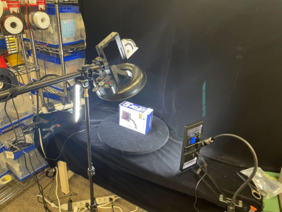
\includegraphics[width=1.0\linewidth]{images/dataset1.png}
		\caption{Use turn-table to capture images of objects from multiple angles.}
	\end{subfigure}
	\begin{subfigure}[t]{0.42\linewidth}
		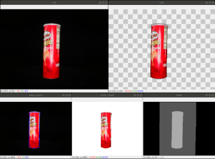
\includegraphics[width=1.0\linewidth]{images/dataset2.png}
		\caption{Crop object images using GUI.}
	\end{subfigure}
	\vfill
	\begin{subfigure}[t]{0.42\linewidth}
		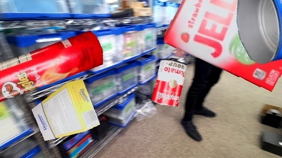
\includegraphics[width=1.0\linewidth]{images/dataset3.png}
		\caption{Generate composite images.}
	\end{subfigure}
	\begin{subfigure}[t]{0.42\linewidth}
		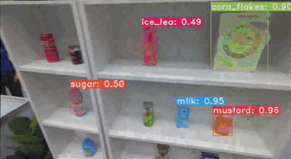
\includegraphics[width=1.0\linewidth]{images/dataset4.png}
		\caption{Object recognition with the model trained on composite images.}
	\end{subfigure}
	\caption{Dataset creation process.}
	\label{fig:dataset}
\end{figure}

\subsection{Speech Recognition And Interaction}

We use EfficientWord-Net\cite{efficientnet} to detect hotword to initiate the conversion.
Once engaged, we employed Google Dialogflow for conversation, which can interpret spoken phrases and generate relevant responses based on our predefined conversational settings.
For vocal output, we use Google Text-To-Speech.

In addition to the current pipeline, we are also exploring the integration of ChatGPT\cite{openai2023gpt4} as a potential replacement for Google Dialogflow to enrich SOAR’s conversational capabilities.
To facilitate this transition, we use Silero VAD\cite{SileroVAD} to segment the voice signals and Whisper\cite{radford2022robust} to convert speech to text.


\section{Contribution}
SoftBank Corp. has continued to sponsor various robotic competitions\footnote{\url{https://wrs.nedo.go.jp/en/sponsor2020/}}\footnote{\url{https://tsukubachallenge.jp/2023/organization/sponsors}} and conferences\footnote{\url{https://ac.rsj-web.org/2023/}}\footnote{\url{https://roscon.ros.org/jp/2023/}} to advocate human-robot interaction research.
Our sister company, SoftBank Robotics Corp. is a long-term global sponsor for RoboCup, which further exemplifies our commitment to advancing robotic technologies and education.
Despite our low direct scientific contribution, SOAR, our current prototype, represents our venture into supporting the research commcomponenty and industry by offering a platform for research and study.
While it is still in development, SOAR is designed with the future in mind, a testament to our initiative in paving the way for affordable and customizable robots, which we believe will make significant contributions to both academic research and practical applications.

\section{Conclusions and future work}
In this paper, we presented our currently developing robot SOAR which will participate in the RoboCup@Home Open Platform League.
We detailed the hardware specification and introduced several software modules, such as object recognition and speech recognition, which we will continue to refine to tackle the tasks in RoboCup @Home for our future work.
By enhancing SOAR’s capabilities in real-world interaction, we aim to contribute not just a flexible and affordable platform but also a robust platform for research and commercial use.


%%%%%%%%%%%%%%%%%%%%%%%%%%%%%%%%%%%%%%%%%%%%%%%%%%%%%%%%%%%%%%%%%%%%%%%%%%%%%%%%%%%%
%
% Bibliography
%
%%%%%%%%%%%%%%%%%%%%%%%%%%%%%%%%%%%%%%%%%%%%%%%%%%%%%%%%%%%%%%%%%%%%%%%%%%%%%%%%%%%%

\bibliographystyle{unsrt}
\bibliography{bibliography}

\clearpage{}

%%%%%%%%%%%%%%%%%%%%%%%%%%%%%%%%%%%%%%%%%%%%%%%%%%%%%%%%%%%%%%%%%%%%%%%%%%%%%%%%%%%%
%
% Robot Specifications
%
%%%%%%%%%%%%%%%%%%%%%%%%%%%%%%%%%%%%%%%%%%%%%%%%%%%%%%%%%%%%%%%%%%%%%%%%%%%%%%%%%%%%

\robospecs{}
%CHKTEX-FILE 46

\section*{SOAR Hardware Description}%
\label{sec:annex-OPL}
% In this section briefly describe the software and hardware of the robot

\setlength\intextsep{0pt}
\begin{wrapfigure}[10]{r}{0.3\textwidth}
	\centering
	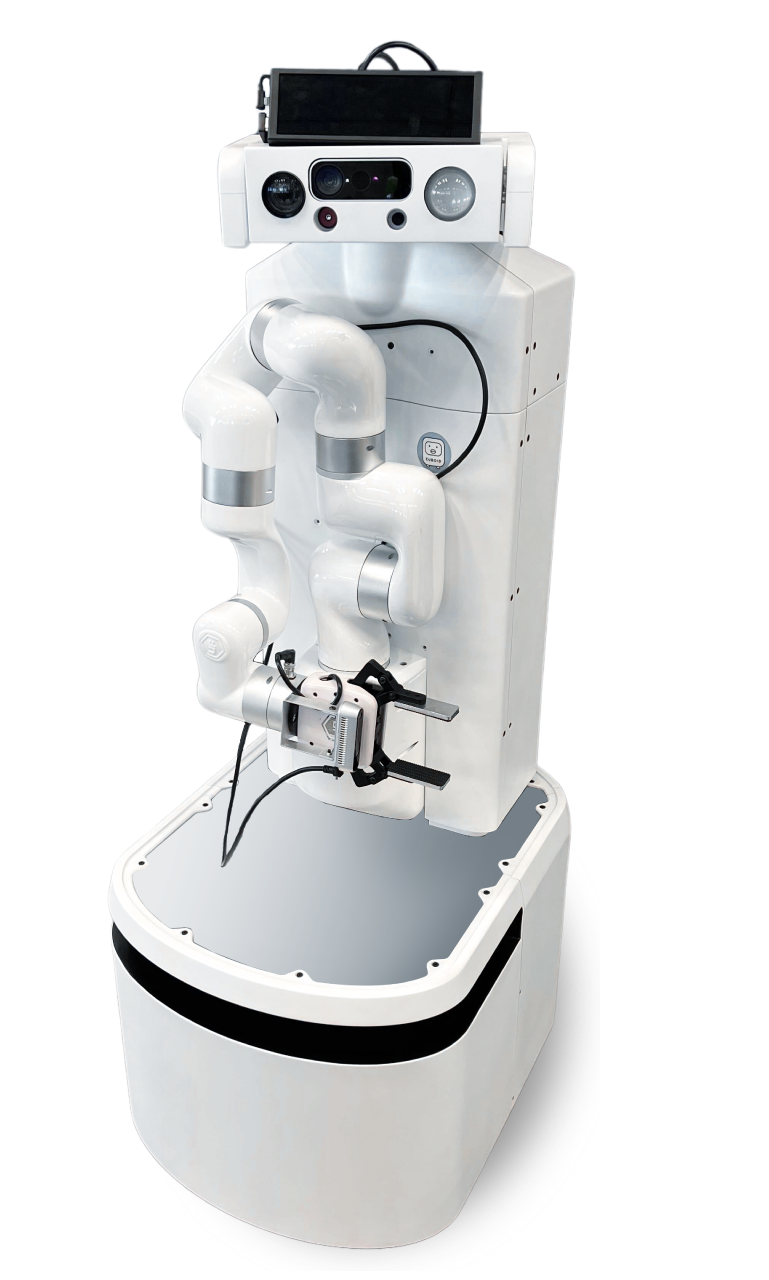
\includegraphics[width=0.4\textwidth]{images/soar.png}
	%\caption{Robot SOAR}%
	\label{fig:soar}
\end{wrapfigure}

Specifications are as follows:

\begin{itemize}
	\item Base: differential drive, 0.83 m/s max speed.
	\item Dimensions: (w) 550 mm (d) 650 mm (h) 1360 mm - 1770 mm
	\item Weight: 92 kg
	\item Arm: 8 DOF (1 DOF torso, 7 DOF manipulator)
	\item Sensors:
	      \begin{itemize}
		      \item Mobile Base:
		            \begin{itemize}
			            \item Hinson LE-50621 LiDAR
			            \item N100 9-axis IMU
		            \end{itemize}
		      \item Head:
		            \begin{itemize}
			            \item Azure Kinect RGB-D camera
			            \item ECM-SP10 microphone
			            \item JM800S-30-360X zoom camera
			            \item Seek Thermal CompactPRO Fast Frame
		            \end{itemize}
		      \item Arm:
		            \begin{itemize}
			            \item Realsense D435 RGB-D camera
		            \end{itemize}
	      \end{itemize}
	\item PC: Intel NUC (NUC11PHKi7C)
	\item Display: THANKO C-79D21B
	\item Speaker: YAMAHA VXS1MLB
\end{itemize}

\section*{SOAR Software Description}
% Please describe in this section the software you are using to control your robot. Consider the following example:

SOAR use the following software components:

\begin{itemize}
	\item Platform: Ubuntu 20.04 ROS Noetic
	\item Navigation: ROS Navigation Stack, EBand local planner
	\item Arm Motion Planner: MoveIt ROS package
	\item Object Recognition:
	      \begin{itemize}
		      \item YOLOv8
		      \item \text{jsk\_pcl\_ros} ROS package
	      \end{itemize}
	\item Behavior Architecture: SMACH ROS package
	\item Hotword: EfficientWord-Net
	\item Speech Recognition: Google Dialogflow
	\item Speech Generation: Google Text-To-Speech
	\item Person Recognition: \text{spencer\_people\_tracking} ROS package
\end{itemize}


\nocite{*}

\end{document}
